
\chapter{Benchmarking a Linux platform}

Benchmarking is the process of measuring the performance of a system. It is a critical step in the process of designing and deploying a system. 
It is important for:
\begin{itemize}
    \item \textbf{Maximize efficiency}: understanding how the server utilizes the CPU, memory, storage and network resources allows for fine-tuning and making better use of the hardwarre full potential.
    \item \textbf{Cost optimization}: understanding the performance of the system allows to make better decisions on the hardware to buy.
    \item \textbf{Troubleshooting issues}: benchmarking can help to identify bottlenecks and performance issues.
    \item \textbf{Security}: benchmarking can help to identify security issues.
    \item \textbf{Comparing systems}: benchmarking can help to compare different systems.
\end{itemize}

\section{Components to test}

There are a lot of tools available on the Internet that can perform
system testing on Linux. We can use them to run different tests and
benchmark various components, such as the Central Processing
Unit (CPU), the Graphics Processing Unit (GPU), memory, database,
and more.

\begin{figure}[H]
    \centering
    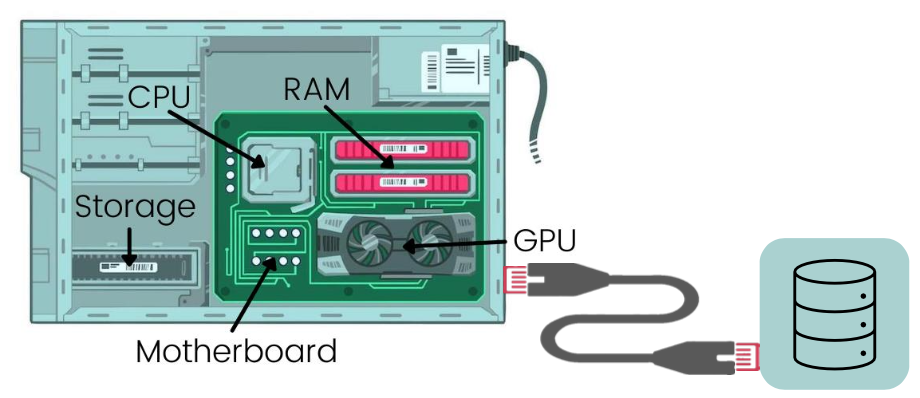
\includegraphics[width=0.7\textwidth]{assets/fig33.png}
    \caption{Components to test}
\end{figure}

\begin{itemize}
    \item \textbf{CPU}: the CPU handles all computational tasks. Measuring its performances helps in understanding how efficiently it handles processes and threads, or whether there are bottlenecks in processing power. 
        \begin{itemize}
            \item stress-ng
            \item sysbench
            \item htop 
            \item mpstat 
            \item HPL 
            \item HPCG 
            \item SPEC
        \end{itemize}
    \item \textbf{Memory (RAM)}: the memory is used to store data and instructions that are currently in use. Measuring its performances helps in understanding how efficiently it handles data and instructions, or whether there are bottlenecks in memory usage.
        \begin{itemize}
            \item stress-ng
            \item memtester
            \item memtest86
            \item valgrind
            \item cachegrind
            \item callgrind
        \end{itemize}
    \item \textbf{Dist I/O and Storage}: the storage is used to store data and instructions that are not currently in use. Measuring its performances helps in understanding how efficiently it handles data and instructions, or whether there are bottlenecks in storage usage.
        \begin{itemize}
            \item fio
            \item ioping
            \item dd
            \item hdparm
            \item bonnie++
            \item iozone
        \end{itemize}
    \item \textbf{Network}: the network is used to transfer data and instructions between different systems. Measuring its performances helps in understanding how efficiently it handles data and instructions, or whether there are bottlenecks in network usage.
        \begin{itemize}
            \item iperf
            \item netperf
            \item nttcp
            \item ping
            \item traceroute
            \item mtr
        \end{itemize}
\end{itemize}


\section{Benchmarking tools}

\subsection{HP Linpack (HPL)}

This is the most famous HPC benchmark, used for the "Top500" ranking. 
It is a software package that solves a random system of linear equations using Gaussian elimination (matrix is dense).

For a given problem size N, HPL performs floating point operations proportional
to N*N*N operations while performing memory reads and write proportional to
N*N.
That means, if the problem size doubles, the number of floating-point operations
increases by a factor of 8 while the number of memory operations only grows by
a factor of 4.
This property of HPL means that it performs very well on systems that have many
flop functional units relative to data movement support. The result is that HPL
tends to represent a very optimistic performance prediction that can only be
matched by a small number of real scientific applications.

\subsection{High Performance Conjugate Gradient (HPCG)}

HPCG uses a simple implementation of the Conjugate Gradients and multigrid
algorithms. It generates and uses sparse data structures that have a very low
compute-to-data-movement ratio.

HPCG has a floating-point operations rate proportional to N and a memory access
rate also proportional to N.
This property means that HPCG performance is strongly influenced by memory
bandwidth.

\section{Tests}

\subsection{CPU}

The CPU is responsible for executing all the
processes, calculations, and tasks. A server’s
overall speed, responsiveness, and ability to
handle concurrent workloads are highly
dependent on the efficiency and power of its
CPU.

In a virtualized environment, CPU testing becomes even more critical since
physical CPU resources are shared between the virtual machines (VMs)
running on the host. The virtual CPUs (vCPUs) allocated to each VM must be
carefully monitored to ensure that the host and all guest VMs operate
efficiently without resource contention.

To test it, we consider the Floating Point Operations Per Second (FLOPS):
$$
FLOPS = \frac{Number\ of\ floating\ point\ operations}{Time}
$$

Floating point operations per clock cycle per core is CPU dependent. 

When testing CPU performance, several key metrics provide insight into how well the CPU handles the system's wordload. 

\begin{itemize}
    \item \textbf{CPU utilization}: the percentage of time the CPU is busy processing instructions.
    \item \textbf{CPU load}: the number of processes in the run queue.
    \item \textbf{CPU temperature}: the temperature of the CPU.
    \item \textbf{CPU frequency}: the frequency of the CPU.
    \item \textbf{CPU cache}: the cache of the CPU.
    \item \textbf{CPU Wait Time}: the time the CPU is waiting for I/O operations to complete.
\end{itemize}

Some tools to test the CPU are:
\begin{enumerate}
    \item \textbf{Baseline tests}: Start by measuring CPU performance under typical workloads to establish a baseline.
    This allows you to understand how the CPU performs under normal conditions. Use as example \texttt{HPL} (see \href{https://hpl-calculator.sourceforge.net/}{HPL Calculator}).
    \item \textbf{Stress tests}: Push the CPU to its limits to see how it performs under heavy workloads. Use as example \texttt{stress-ng} or \texttt{sysbench}. It can create stress on CPU, cache and memory.
    \item \textbf{htop}: An interactive system monitor that provides real-time information on CPU utilization,
    load average, and the number of running processes. It visually represents per-core
    utilization. Simply run \texttt{htop} from the command line.
    \item \textbf{mpstat}: A command-line utility that provides real-time CPU statistics. It displays
    information on CPU utilization, idle time, and wait time. Run \texttt{mpstat} from the
    command line.
\end{enumerate}

Analysis on the results:
\begin{itemize}
    \item \textbf{CPU utilization}: the percentage of time the CPU is busy processing instructions. A high CPU utilization indicates that the CPU is working hard to process instructions. A low CPU utilization indicates that the CPU is not working hard to process instructions.
    \item \textbf{CPU load}: the number of processes in the run queue. A high CPU load indicates that there are many processes waiting to be executed. A low CPU load indicates that there are few processes waiting to be executed.
    \item \textbf{High Context Switches}: A high number of context switches indicates that the CPU is switching between processes frequently. This can lead to performance issues.
    \item \textbf{High Interrupts}: A high number of interrupts indicates that the CPU is handling a large number of hardware interrupts. This can lead to performance issues.
    \item \textbf{vCPU Overcommitment}: Overcommitting vCPUs can lead to performance issues. Make sure that the number of vCPUs allocated to a VM does not exceed the number of physical cores on the host.
\end{itemize}

\subsection{Memory}

Memory is used to store data and instructions that are currently in use. Measuring its performance helps in understanding how efficiently it handles data and instructions, or whether there are bottlenecks in memory usage.

Memory is one of the most vital components of a server,
affecting how quickly applications can access and manipulate
data. Inadequate memory resources, poor memory
management, or issues with memory speed can lead to severe
performance bottlenecks. For example, if the system runs out of
physical memory, it may start using swap space (disk-based
memory), which can significantly degrade performance.

Testing memory performance ensures that the system can handle workloads
effectively without encountering delays due to insufficient or slow memory. This is
particularly important in environments running databases, virtual machines, or in-
memory data stores (like Redis).

When testing memory performance, several key metrics provide insight into how well the memory handles the system's workload.
\begin{itemize}
    \item \textbf{Memory utilization}: the percentage of memory that is being used.
    \item \textbf{Memory load}: the number of processes that are using memory.
    \item \textbf{Memory latency}: the time it takes to access memory.
    \item \textbf{Memory bandwidth}: the rate at which data can be read from or written to memory.
    \item \textbf{Memory errors}: the number of memory errors that occur.
    \item \textbf{Cache Hit/Miss Ratio}: the ratio of cache hits to cache misses.
\end{itemize}

Some tools to test the memory are:
\begin{enumerate}
    \item \textbf{Baseline tests}: Start by measuring memory performance under typical workloads to establish a baseline. This allows you to understand how the memory performs under normal conditions. Use as example \texttt{memtester} or \texttt{memtest86}.
    \item \textbf{Stress tests}: Push the memory to its limits to see how it performs under heavy workloads. Use as example \texttt{stress-ng} or \texttt{memtester}.
    \item \textbf{valgrind}: A memory debugging tool that can be used to profile memory usage and detect memory leaks. Run \texttt{valgrind} from the command line.
    \item \textbf{cachegrind}: A cache profiling tool that can be used to profile cache usage. Run \texttt{cachegrind} from the command line.
    \item \textbf{callgrind}: A call graph profiling tool that can be used to profile function calls. Run \texttt{callgrind} from the command line.
\end{enumerate}

Analysis on the results:
\begin{itemize}
    \item \textbf{Memory utilization}: the percentage of memory that is being used. A high memory utilization indicates that the memory is being used heavily. A low memory utilization indicates that the memory is not being used heavily.
    \item \textbf{Memory load}: the number of processes that are using memory. A high memory load indicates that there are many processes using memory. A low memory load indicates that there are few processes using memory.
    \item \textbf{Memory latency}: the time it takes to access memory. A low memory latency indicates that memory access is fast. A high memory latency indicates that memory access is slow.
    \item \textbf{Memory bandwidth}: the rate at which data can be read from or written to memory. A high memory bandwidth indicates that memory access is fast. A low memory bandwidth indicates that memory access is slow.
    \item \textbf{Memory errors}: the number of memory errors that occur. A high number of memory errors indicates that there are issues with memory.
    \item \textbf{Cache Hit/Miss Ratio}: the ratio of cache hits to cache misses. A high cache hit/miss ratio indicates that the cache is being used effectively. A low cache hit/miss ratio indicates that the cache is not being used effectively.
\end{itemize}

\subsection{Disk I/O and Storage}

Disk I/O (Input/Output) is a critical factor in server
performance, especially for databases, web servers, and
applications that rely on frequent disk access. Slow disk
performance can lead to bottlenecks where applications
are waiting on data retrieval or writing operations,
causing delays and system slowdowns. In addition,
storage subsystems like RAID arrays and SSDs have
different performance characteristics that must be
optimized for the server’s workload.

Cloud and Virtualized environments also introduce additional complexity since
multiple virtual machines may share the same physical storage, increasing the
potential for resource contention.

When testing disk I/O and storage performance, several key metrics provide insight into how well the storage subsystem handles the system's workload.

\begin{itemize}
    \item \textbf{Read/Write Throughput}: the rate at which data can be read from or written to disk.
    \item \textbf{Read/Write Latency}: the time it takes to read from or write to disk.
    \item \textbf{IOPS (Input/Output Operations Per Second)}: the number of read/write operations that can be performed per second.
    \item \textbf{Disk Queue Length}: the number of read/write requests that are waiting to be processed.
    \item \textbf{Disk Errors}: the number of disk errors that occur.
    \item \textbf{SSD vs HDD}: the performance difference between SSDs and HDDs.
\end{itemize}

Some tools to test the disk I/O and storage are:
\begin{enumerate}
    \item \textbf{Baseline tests}: Start by measuring disk I/O and storage performance under typical workloads to establish a baseline. This allows you to understand how the storage subsystem performs under normal conditions. Use as example \texttt{fio} or \texttt{dd}.
    \item \textbf{Stress tests}: Push the disk I/O and storage to its limits to see how it performs under heavy workloads. Use as example \texttt{fio} or \texttt{dd}.
    \item \textbf{ioping}: A disk I/O latency tool that can be used to measure disk I/O latency. Run \texttt{ioping} from the command line.
    \item \textbf{hdparm}: A disk performance tool that can be used to measure disk performance. Run \texttt{hdparm} from the command line.
    \item \textbf{bonnie++}: A disk benchmarking tool that can be used to measure disk performance. Run \texttt{bonnie++} from the command line.
    \item \textbf{iozone}: A disk benchmarking tool that can be used to measure disk performance. Run \texttt{iozone} from the command line.
\end{enumerate}

Analysis on the results:
\begin{itemize}
    \item \textbf{Read/Write Throughput}: the rate at which data can be read from or written to disk. A high read/write throughput indicates that the disk I/O and storage subsystem is performing well. A low read/write throughput indicates that the disk I/O and storage subsystem is not performing well.
    \item \textbf{Read/Write Latency}: the time it takes to read from or write to disk. A low read/write latency indicates that disk I/O and storage access is fast. A high read/write latency indicates that disk I/O and storage access is slow.
    \item \textbf{IOPS (Input/Output Operations Per Second)}: the number of read/write operations that can be performed per second. A high IOPS indicates that the disk I/O and storage subsystem is performing well. A low IOPS indicates that the disk I/O and storage subsystem is not performing well.
    \item \textbf{Disk Queue Length}: the number of read/write requests that are waiting to be processed. A high disk queue length indicates that there are many read/write requests waiting to be processed. A low disk queue length indicates that there are few read/write requests waiting to be processed.
    \item \textbf{Disk Errors}: the number of disk errors that occur. A high number of disk errors indicates that there are issues with the disk I/O and storage subsystem.
    \item \textbf{SSD vs HDD}: the performance difference between SSDs and HDDs. SSDs are faster than HDDs and have lower latency.
\end{itemize}




